\subsubsection{The 2D annulus benchmark}
\label{sec:cookbooks-annulus}

\textit{This section was contributed by C. Thieulot and E. G. Puckett.}

This benchmark is based on a manufactured solution in which an analytical solution to the
isoviscous incompressible Stokes equations is derived in an annulus geometry.
The velocity and pressure fields are as follows:

\begin{eqnarray}
v_r(r,\theta)     &=&  g(r) k \sin(k\theta), \\
v_\theta(r,\theta)&=&  f(r) \cos(k \theta), \\
p(r,\theta)       &=&  k h(r) \sin(k \theta), \\
\rho (r,\theta)   &=& \aleph(r) k \sin (k \theta),
\end{eqnarray}
with
\begin{eqnarray}
f(r)&=&Ar+B/r, \\
g(r) &=& \frac{A}{2}r  +  \frac{B}{r} \ln r + \frac{C}{r}, \\
h(r)&=& \frac{2g(r)-f(r)}{r},  \\
\aleph(r) &=& g'' - \frac{g'}{r}  - \frac{g}{r^2} (k^2 - 1)  + \frac{f}{r^2}   + \frac{f'}{r}, \\
A &=& -C\frac{2(\ln R_1 - \ln R_2)} { R_2^2 \ln R_1  - R_1^2 \ln R_2}, \\
B &=& -C \frac{R_2^2-R_1^2}{R_2^2 \ln R_1 - R_1^2 \ln R_2}.
\end{eqnarray}

The parameters $A$ and $B$ are chosen so that $v_r(R_1)=v_r(R_2)=0$, i.e.
the velocity is tangential to both inner and outer surfaces.
The gravity vector is radial and of unit length.

The parameter $k$ controls the number of convection cells present in the domain,
as shown in Fig.~\ref{fig:annulus-vp}.

\begin{figure}
\centering
\includegraphics[width=.9\textwidth]{cookbooks/benchmarks/annulus/doc/pressures.png}
\includegraphics[width=.9\textwidth]{cookbooks/benchmarks/annulus/doc/density.png}
\includegraphics[width=.9\textwidth]{cookbooks/benchmarks/annulus/doc/velocities2.png}
\caption{\it Pressure, density and velocity fields for $k=0,1,2,3$ for the 2D annulus benchmark.}
\label{fig:annulus-vp}
\end{figure}

In the present case, we set $R_1=1$, $R_2=2$ and $C=-1$. Fig.~\ref{fig:annulus-errors} shows the
velocity and pressure errors in the $L_2$-norm as a function of the mesh size $h$ (taken in this case
as the radial extent of the elements). As expected we recover a third-order convergence rate for the velocity
and a second-order convergence rate for the pressure.

\begin{figure}
\centering
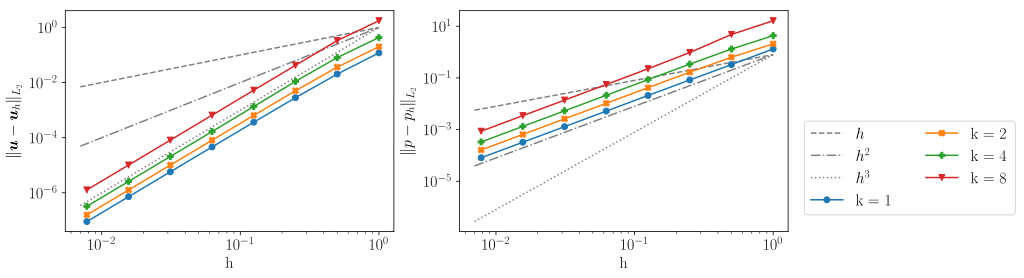
\includegraphics[width=.7\textwidth]{cookbooks/benchmarks/annulus/doc/errors_annulus.pdf}
\caption{\it Velocity and pressure errors in the $L_2$-norm as a function of the mesh size for the 2D annulus benchmark.}
\label{fig:annulus-errors}
\end{figure}
